\documentclass[12pt,a4paper]{article}

\usepackage[utf8]{inputenc} \usepackage[T1]{fontenc} \usepackage{graphicx}
\usepackage{longtable} \usepackage{tabularx} \usepackage{float}
\usepackage{wrapfig} \usepackage{soul} \usepackage{amssymb}
\usepackage{hyperref} \usepackage{caption} \usepackage{subcaption}
\usepackage{pdfpages} \usepackage{sidecap}


\parindent 0in \usepackage[spanish]{babel}
\setlength{\parskip}{0.5\baselineskip} \usepackage{fullpage}
\usepackage{multirow} \usepackage{multicol} \usepackage{framed}
\usepackage{listings} \usepackage{enumerate}

\usepackage{appendix} \usepackage{setspace} \usepackage{amsmath}


%% DEFINICIONES
\newcommand{\TODO}[1]{{\huge \color{red} \textbf{TODO: }#1 }}
\newcommand{\todo}[1]{{\large \color{red} \textbf{TODO: }#1 }}


\title{Práctica 2. \\ Geometría computacional} 

\author{Luis María Costero Valero (lcostero@ucm.es)\\ Jesús Doménech
  Arellano (jdomenec@ucm.es) \\ Jennifer Hernández Bécares (jennhern@ucm.es)}
\date{Marzo 2015}

\begin{document}
\maketitle

\todo{Revisar el párrafo y cambiar el nombre de los archivos (algo como P2\_intervactivo.py}
En esta práctica entregamos dos versiones del código, la primera en el
archivo P2.py y la segunda en P2\_chulo.py. La diferencia es que la
segunda versión permite meter las condiciones iniciales de la
geodésica pinchando en el plot. Dado que el código se complica,
entregamos la versión sin esta mejora para facilitar la corrección de
la práctica.

\begin{enumerate}
\item Dado el toro de revolución usual, dibújese sobre el mismo una
  geodésica cuya traza sea uno de los dos círculos generadores.\\
  Dibujamos el toro con $r = 2.0$ y $a = 5.0$ \\
  Para el círculo generador tomamos de condiciones iniciales:
  \begin{itemize}
  \item $(u_0, v_0) = (0, 0)$
  \item $(u'_0, v'_0) = (0, 1)$
  \end{itemize}

  \begin{center}
    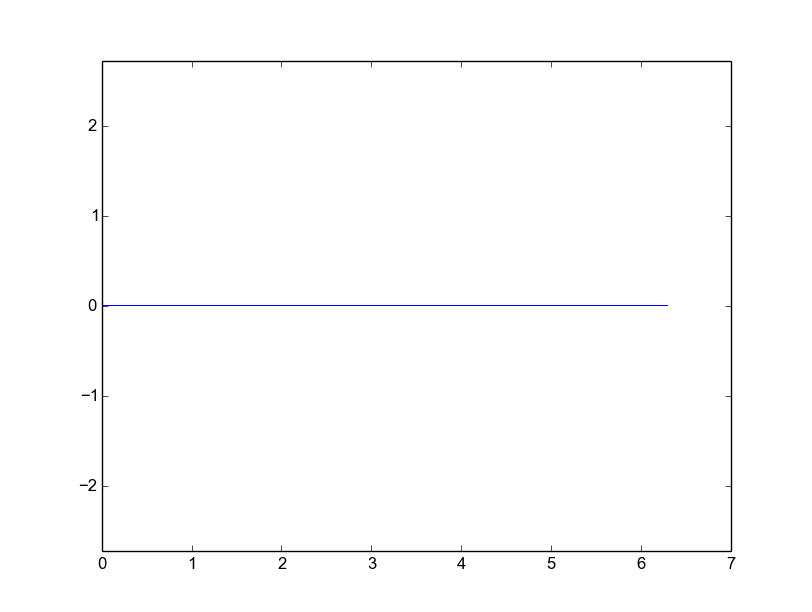
\includegraphics[width=0.4\textwidth]{./img/circulo1_trace.png}
    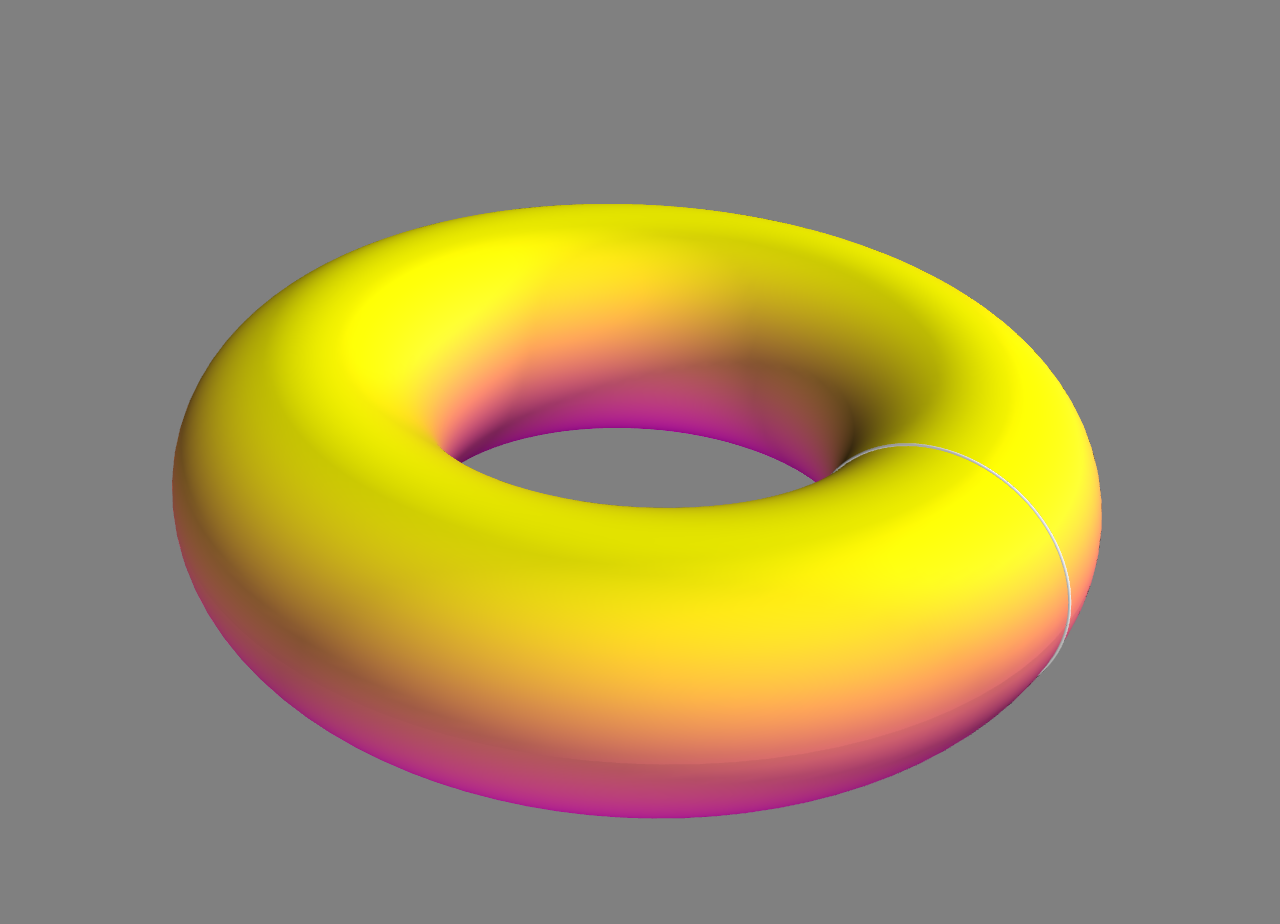
\includegraphics[width=0.4\textwidth]{./img/circulo1_surface.png}
  \end{center}

  El otro cículo generador se obtiene al establecer las derivadas iniciales
  como\\ $(u'_0, v'_0) = (1, 0)$

\item Dibújese sobre el toro una geodésica periódica. Dibújese sobre
  el toro una geodésica no periódica. Opcional: ¿Sabrías obtenener una
  geodésica que sea densa sobre todo el toro?
  \begin{enumerate}
  \item Periódica: 
  \begin{center}
    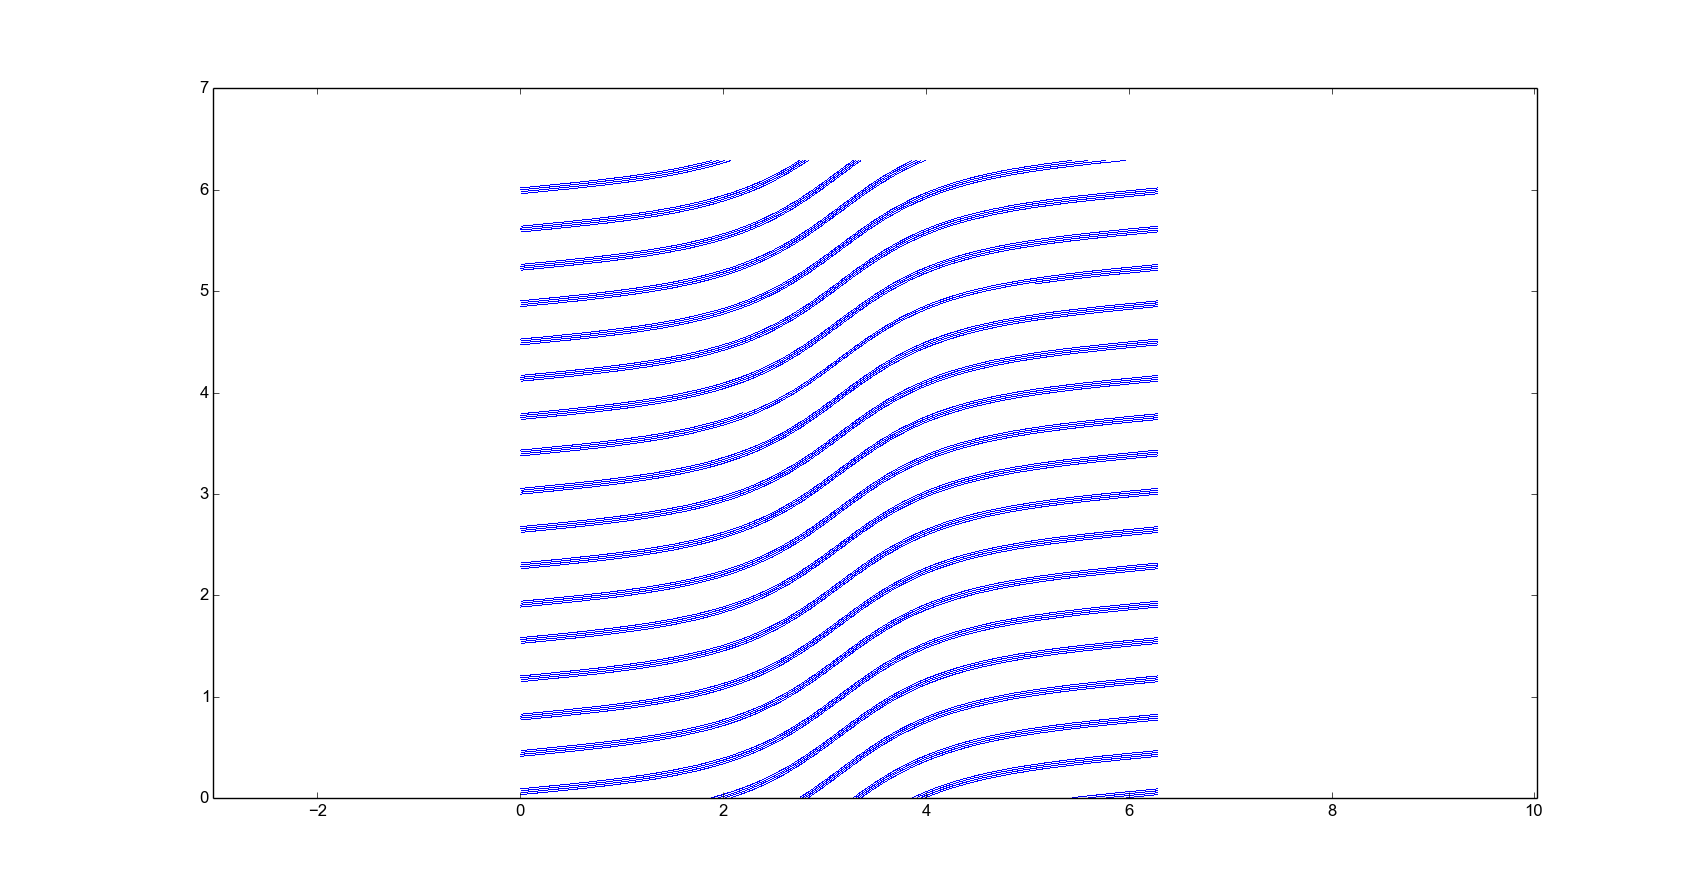
\includegraphics[width=0.4\textwidth]{./img/periodica_trace.png}
    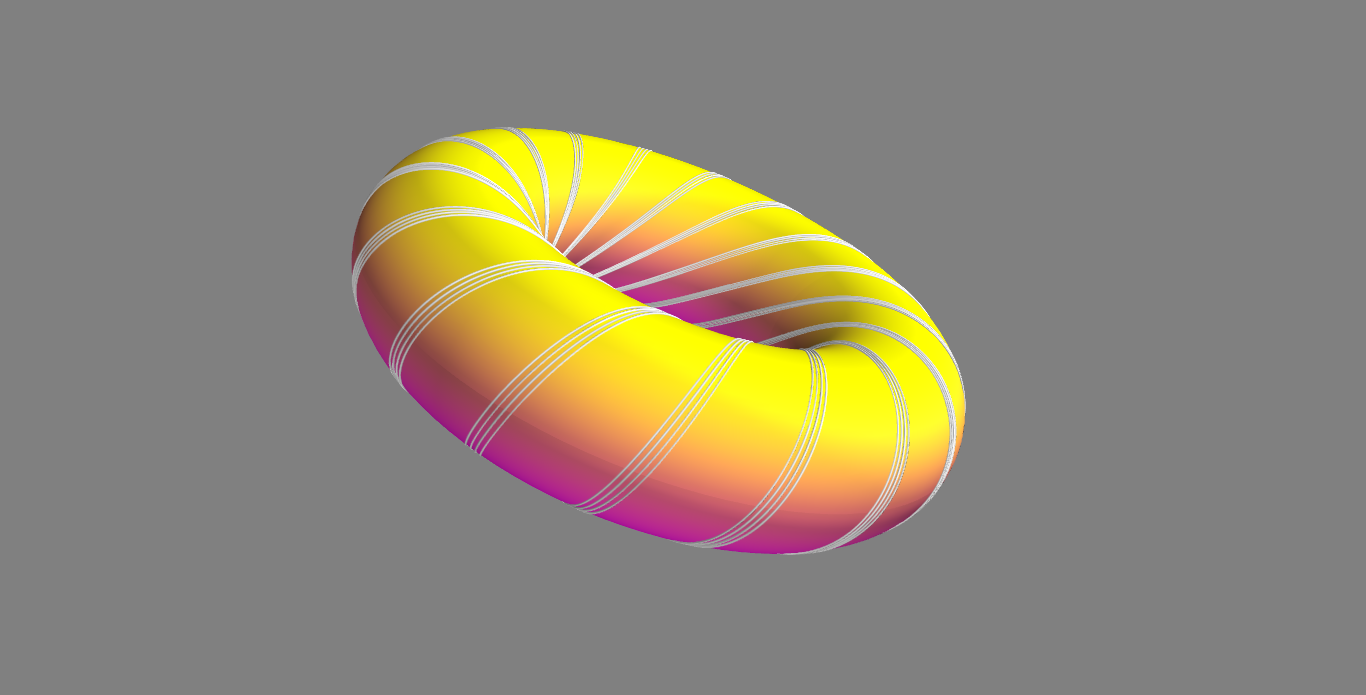
\includegraphics[width=0.4\textwidth]{./img/periodica_surface.png}
  \end{center}
  \item Periódica: Por ejemplo el caso del círculo generador.
  \item No periódica: ¿EXISTE? ¿está bien esta?
    \begin{itemize}
    \item $u(t_0) = \pi$
    \item $v(t_0) = 0.0$
    \item $u'(t_0) = 1.0$
    \item $v'(t_0) = 1.0$
    \end{itemize}
  \item Opcional: Ni idea
    \begin{itemize}
    \item $u(t_0) = $
    \item $v(t_0) = $
    \item $u'(t_0) = $
    \item $v'(t_0) = $
    \end{itemize}
  \end{enumerate}
\item Modelo de plano hiperbólico dado por el semiplano de
  Poincaré. Considérese la primera forma fundamental en el semiplano
  $v>0$ dada por $E = G = \frac{1}{v^{2}}$ y $G = 0$. Dibújense sus
  geodésicas. 
  \begin{center}
    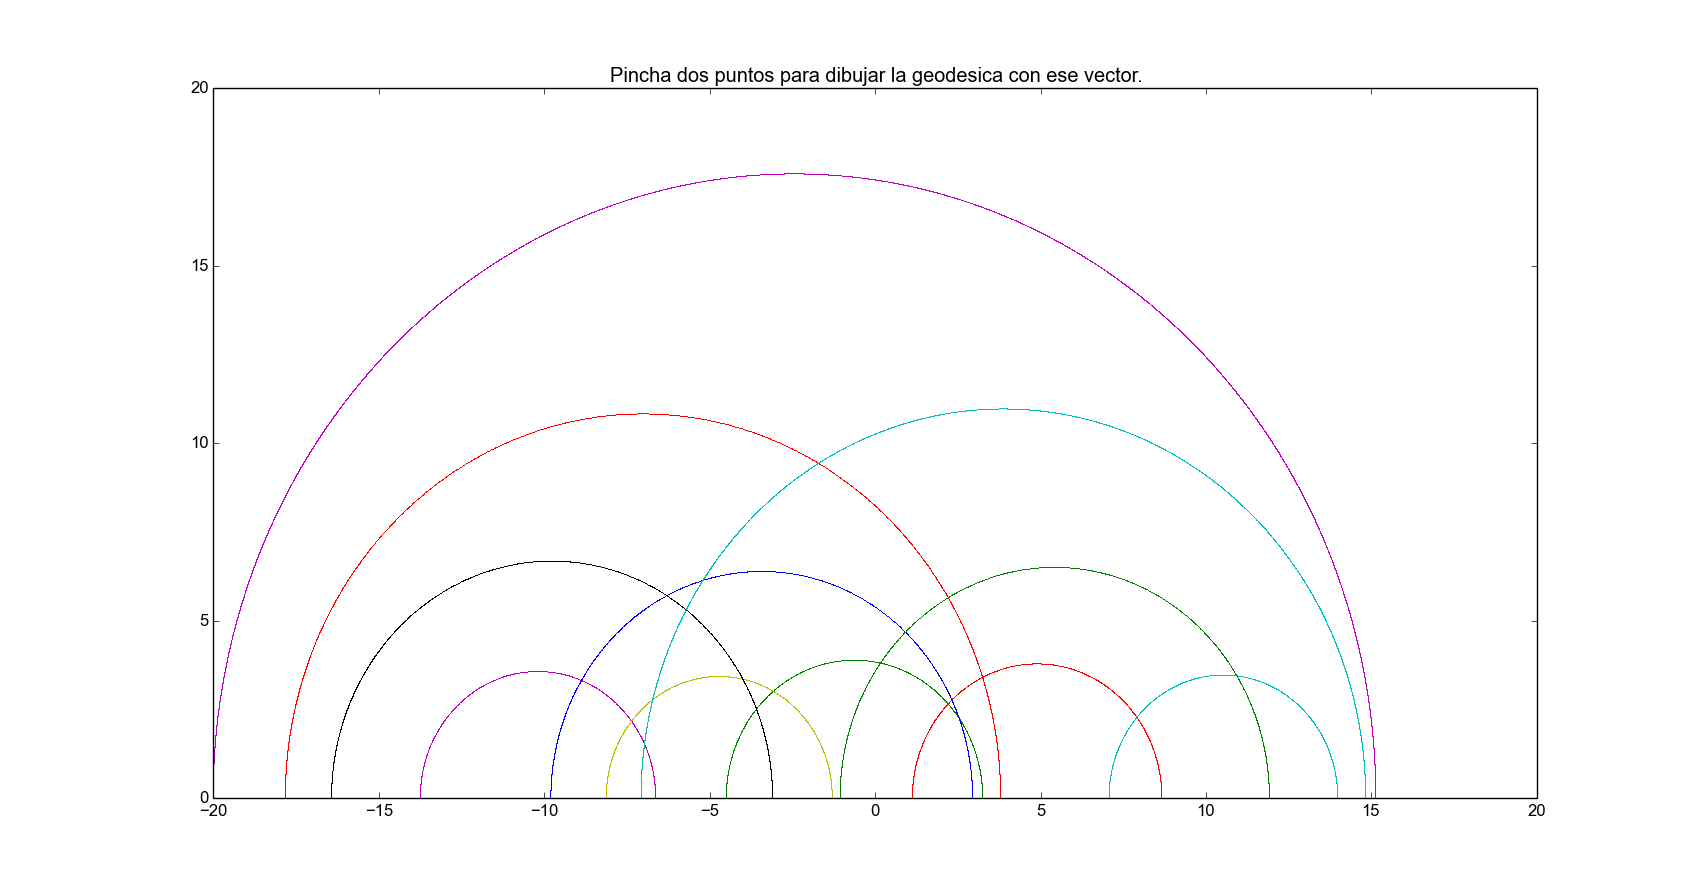
\includegraphics[width=0.8\textwidth]{./img/poincare.png}
  \end{center}

\end{enumerate}
\end{document}
